\documentclass[]{krantz}
\usepackage{lmodern}
\usepackage{amssymb,amsmath}
\usepackage{ifxetex,ifluatex}
\usepackage{fixltx2e} % provides \textsubscript
\ifnum 0\ifxetex 1\fi\ifluatex 1\fi=0 % if pdftex
  \usepackage[T1]{fontenc}
  \usepackage[utf8]{inputenc}
\else % if luatex or xelatex
  \ifxetex
    \usepackage{mathspec}
  \else
    \usepackage{fontspec}
  \fi
  \defaultfontfeatures{Ligatures=TeX,Scale=MatchLowercase}
\fi
% use upquote if available, for straight quotes in verbatim environments
\IfFileExists{upquote.sty}{\usepackage{upquote}}{}
% use microtype if available
\IfFileExists{microtype.sty}{%
\usepackage{microtype}
\UseMicrotypeSet[protrusion]{basicmath} % disable protrusion for tt fonts
}{}
\usepackage[margin=1in]{geometry}
\usepackage{hyperref}
\PassOptionsToPackage{usenames,dvipsnames}{color} % color is loaded by hyperref
\hypersetup{unicode=true,
            pdftitle={Limitations of Interpretable Machine Learning Methods},
            colorlinks=true,
            linkcolor=Maroon,
            citecolor=Blue,
            urlcolor=Blue,
            breaklinks=true}
\urlstyle{same}  % don't use monospace font for urls
\usepackage{color}
\usepackage{fancyvrb}
\newcommand{\VerbBar}{|}
\newcommand{\VERB}{\Verb[commandchars=\\\{\}]}
\DefineVerbatimEnvironment{Highlighting}{Verbatim}{commandchars=\\\{\}}
% Add ',fontsize=\small' for more characters per line
\usepackage{framed}
\definecolor{shadecolor}{RGB}{248,248,248}
\newenvironment{Shaded}{\begin{snugshade}}{\end{snugshade}}
\newcommand{\KeywordTok}[1]{\textcolor[rgb]{0.13,0.29,0.53}{\textbf{#1}}}
\newcommand{\DataTypeTok}[1]{\textcolor[rgb]{0.13,0.29,0.53}{#1}}
\newcommand{\DecValTok}[1]{\textcolor[rgb]{0.00,0.00,0.81}{#1}}
\newcommand{\BaseNTok}[1]{\textcolor[rgb]{0.00,0.00,0.81}{#1}}
\newcommand{\FloatTok}[1]{\textcolor[rgb]{0.00,0.00,0.81}{#1}}
\newcommand{\ConstantTok}[1]{\textcolor[rgb]{0.00,0.00,0.00}{#1}}
\newcommand{\CharTok}[1]{\textcolor[rgb]{0.31,0.60,0.02}{#1}}
\newcommand{\SpecialCharTok}[1]{\textcolor[rgb]{0.00,0.00,0.00}{#1}}
\newcommand{\StringTok}[1]{\textcolor[rgb]{0.31,0.60,0.02}{#1}}
\newcommand{\VerbatimStringTok}[1]{\textcolor[rgb]{0.31,0.60,0.02}{#1}}
\newcommand{\SpecialStringTok}[1]{\textcolor[rgb]{0.31,0.60,0.02}{#1}}
\newcommand{\ImportTok}[1]{#1}
\newcommand{\CommentTok}[1]{\textcolor[rgb]{0.56,0.35,0.01}{\textit{#1}}}
\newcommand{\DocumentationTok}[1]{\textcolor[rgb]{0.56,0.35,0.01}{\textbf{\textit{#1}}}}
\newcommand{\AnnotationTok}[1]{\textcolor[rgb]{0.56,0.35,0.01}{\textbf{\textit{#1}}}}
\newcommand{\CommentVarTok}[1]{\textcolor[rgb]{0.56,0.35,0.01}{\textbf{\textit{#1}}}}
\newcommand{\OtherTok}[1]{\textcolor[rgb]{0.56,0.35,0.01}{#1}}
\newcommand{\FunctionTok}[1]{\textcolor[rgb]{0.00,0.00,0.00}{#1}}
\newcommand{\VariableTok}[1]{\textcolor[rgb]{0.00,0.00,0.00}{#1}}
\newcommand{\ControlFlowTok}[1]{\textcolor[rgb]{0.13,0.29,0.53}{\textbf{#1}}}
\newcommand{\OperatorTok}[1]{\textcolor[rgb]{0.81,0.36,0.00}{\textbf{#1}}}
\newcommand{\BuiltInTok}[1]{#1}
\newcommand{\ExtensionTok}[1]{#1}
\newcommand{\PreprocessorTok}[1]{\textcolor[rgb]{0.56,0.35,0.01}{\textit{#1}}}
\newcommand{\AttributeTok}[1]{\textcolor[rgb]{0.77,0.63,0.00}{#1}}
\newcommand{\RegionMarkerTok}[1]{#1}
\newcommand{\InformationTok}[1]{\textcolor[rgb]{0.56,0.35,0.01}{\textbf{\textit{#1}}}}
\newcommand{\WarningTok}[1]{\textcolor[rgb]{0.56,0.35,0.01}{\textbf{\textit{#1}}}}
\newcommand{\AlertTok}[1]{\textcolor[rgb]{0.94,0.16,0.16}{#1}}
\newcommand{\ErrorTok}[1]{\textcolor[rgb]{0.64,0.00,0.00}{\textbf{#1}}}
\newcommand{\NormalTok}[1]{#1}
\usepackage{longtable,booktabs}
\usepackage{graphicx,grffile}
\makeatletter
\def\maxwidth{\ifdim\Gin@nat@width>\linewidth\linewidth\else\Gin@nat@width\fi}
\def\maxheight{\ifdim\Gin@nat@height>\textheight\textheight\else\Gin@nat@height\fi}
\makeatother
% Scale images if necessary, so that they will not overflow the page
% margins by default, and it is still possible to overwrite the defaults
% using explicit options in \includegraphics[width, height, ...]{}
\setkeys{Gin}{width=\maxwidth,height=\maxheight,keepaspectratio}
\IfFileExists{parskip.sty}{%
\usepackage{parskip}
}{% else
\setlength{\parindent}{0pt}
\setlength{\parskip}{6pt plus 2pt minus 1pt}
}
\setlength{\emergencystretch}{3em}  % prevent overfull lines
\providecommand{\tightlist}{%
  \setlength{\itemsep}{0pt}\setlength{\parskip}{0pt}}
\setcounter{secnumdepth}{5}
% Redefines (sub)paragraphs to behave more like sections
\ifx\paragraph\undefined\else
\let\oldparagraph\paragraph
\renewcommand{\paragraph}[1]{\oldparagraph{#1}\mbox{}}
\fi
\ifx\subparagraph\undefined\else
\let\oldsubparagraph\subparagraph
\renewcommand{\subparagraph}[1]{\oldsubparagraph{#1}\mbox{}}
\fi

%%% Use protect on footnotes to avoid problems with footnotes in titles
\let\rmarkdownfootnote\footnote%
\def\footnote{\protect\rmarkdownfootnote}

%%% Change title format to be more compact
\usepackage{titling}

% Create subtitle command for use in maketitle
\newcommand{\subtitle}[1]{
  \posttitle{
    \begin{center}\large#1\end{center}
    }
}

\setlength{\droptitle}{-2em}

  \title{Limitations of Interpretable Machine Learning Methods}
    \pretitle{\vspace{\droptitle}\centering\huge}
  \posttitle{\par}
    \author{}
    \preauthor{}\postauthor{}
      \predate{\centering\large\emph}
  \postdate{\par}
    \date{2019-05-19}


\begin{document}
\maketitle

{
\hypersetup{linkcolor=black}
\setcounter{tocdepth}{2}
\tableofcontents
}
\listoftables
\listoffigures
\section*{Preface}\label{preface}
\addcontentsline{toc}{section}{Preface}

This project explains the limitations of current approaches in
interpretable machine learning, such as partial dependence plots (PDP,
Accumulated Local Effects (ALE), permutation feature importance,
leave-one-covariate out (LOCO) and local interpretable model-agnostic
explanations (LIME). All of those methods can be used to explain the
behavior and predictions of trained machine learning models. The
interpretation methods might not work well in the following cases:

\begin{itemize}
\tightlist
\item
  if a model models interactions (e.g.~when a random forest is used)
\item
  if features strongly correlate with each other
\item
  if the model does not correctly model causal relationships
\item
  if parameters of the interpretation method are not set correctly
\end{itemize}

\subsection*{Structure of the book}\label{structure-of-the-book}
\addcontentsline{toc}{subsection}{Structure of the book}

TODO

\mainmatter

\section{Introduction}\label{introduction}

Here is some text

\subsection{This is a smaller title}\label{this-is-a-smaller-title}

We have a nice figure in Figure \ref{fig:hello}, and also a table in
Table \ref{tab:iris}.

\begin{Shaded}
\begin{Highlighting}[]
\KeywordTok{par}\NormalTok{(}\DataTypeTok{mar =} \KeywordTok{c}\NormalTok{(}\DecValTok{4}\NormalTok{, }\DecValTok{4}\NormalTok{, }\DecValTok{1}\NormalTok{, .}\DecValTok{1}\NormalTok{))}
\KeywordTok{plot}\NormalTok{(cars, }\DataTypeTok{pch =} \DecValTok{19}\NormalTok{)}
\end{Highlighting}
\end{Shaded}

\begin{figure}
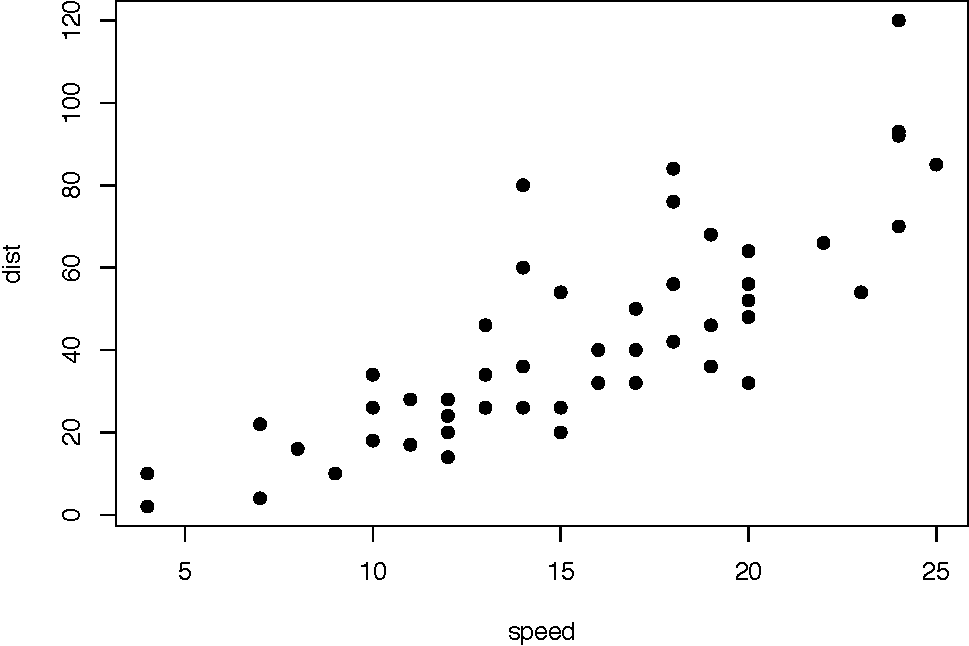
\includegraphics[width=0.9\linewidth]{book_files/figure-latex/hello-1} \caption{Hello World!}\label{fig:hello}
\end{figure}

\begin{Shaded}
\begin{Highlighting}[]
\NormalTok{knitr}\OperatorTok{::}\KeywordTok{kable}\NormalTok{(}
  \KeywordTok{head}\NormalTok{(iris), }\DataTypeTok{caption =} \StringTok{'The boring iris data.'}\NormalTok{,}
  \DataTypeTok{booktabs =} \OtherTok{TRUE}
\NormalTok{)}
\end{Highlighting}
\end{Shaded}

\begin{table}

\caption{\label{tab:iris}The boring iris data.}
\centering
\begin{tabular}[t]{rrrrl}
\toprule
Sepal.Length & Sepal.Width & Petal.Length & Petal.Width & Species\\
\midrule
5.1 & 3.5 & 1.4 & 0.2 & setosa\\
4.9 & 3.0 & 1.4 & 0.2 & setosa\\
4.7 & 3.2 & 1.3 & 0.2 & setosa\\
4.6 & 3.1 & 1.5 & 0.2 & setosa\\
5.0 & 3.6 & 1.4 & 0.2 & setosa\\
5.4 & 3.9 & 1.7 & 0.4 & setosa\\
\bottomrule
\end{tabular}
\end{table}

\section{Partial Dependence Plots (PDP) and Individual Conditional
Expectation
Curves}\label{partial-dependence-plots-pdp-and-individual-conditional-expectation-curves}

\subsection{Partial Dependence Plots}\label{partial-dependence-plots}

\subsection{ICE}\label{ice}

\section{Accumulated Local Effects
(ALE)}\label{accumulated-local-effects-ale}

\section{Permutation Feature Importance and
LOCO}\label{permutation-feature-importance-and-loco}

\subsection{Permutation Feature
Importance}\label{permutation-feature-importance}

\subsection{Leave-One-Covariate-Out
(LOCO)}\label{leave-one-covariate-out-loco}

\section{Local Interpretable Model-agnostic
Explanations}\label{local-interpretable-model-agnostic-explanations}

(\# First merge start)

So far all of the interpretation methods presented in this book are
refer to the global scope of the trained model. However, none really
gives the opportunity to interpret a model via single predictions on
their own. This is where the method LIME (local interpretable
model-agnostic explanations) comes into play. LIME is a variant of
so-called surrogate models. Surrogate models aim to imitate the black
box prediction behaviour of a machine learning model. Surrogate models
themselves have a certain feature: they are interpretable. The intuition
is to have an interpretable model that explains the association of the
features \(X\) and the - by the black box model - \emph{predicted}
target \(\hat{y}\). Thus, surrogate models aim to capture the decision
boundaries of the black box model without attempting to model the true
association itself. For example, we may use a neural network to solve a
classification task. While a neural network is anything but
interpretable, we may find that some of the decision boundaries are
reasonably well explained by a logistic regression which in fact yields
interpretable coefficients.

In general there are two kinds of surrogate models: global and local
surrogate models. In this chapter we will focus on the latter ones.

The concept of local surrogate models is heavily tied to \cite{LIME} who
propose local interpretable model-agnostic explanations (LIME).
Different to global surrogate models, local surrogate models such as
LIME aim to rather explain single predictions by interpretable models
than the whole black box model. Using LIME one tries to
\emph{locally interpret} this prediction solely by a new surrogate model
- a \emph{model-agnostic explanation} so to say. This model, also
referred to as explainer, needs to be easiliy interpretable (like a
linear regression model or a decision tree) and thus may of course not
have the adaptability and flexibility of the original black box model.
However, we actually don't care about a global fit in this case. We only
want to have a very local fit of the explainer in the neighbourhood of
the instance to be explained.

So far so good. However, the previous outline was not very specific and
leaves (at least) three questions. First, what should the input of the
explainer be like? Second, what does neighbourhood refer to? Third, what
properties should suitable explainers have?

To better assess these open questions it may be helpful to study the
mathematical defintion of \(LIME\).

The explainer function for a datapoint \(x\) which we aim to interpret
is of the following form:

\begin{equation}
  explainer\left(x\right) = arg\,min_{g \epsilon G} \,\mathcal{L}\left(f, g, \pi_x \right) + \Omega\left(g\right)
\end{equation}

Let's decompose this compact, yet precise definition: \(x\) can be any
arbitrary (new) data that can be represented in the same way as the
original data. Besides the classical tabular data case, we can also
interpret models trained on text data or image data. However, some data
representations (e.g.~word embeddings for text data) are not
human-interpretable and must be replaced by interpretable variants
(e.g.~one-hot-encoded word vectors) for LIME to yield interpretable
results. Additionally, it is important to understand that the explainer
only aims to explain the black box model behaviour and not the data this
model was fit on. The function modelled by the black box model operates
in the complete feature space and can even yield predictions for
instances not seen in the training data. Hence, we want to create more
complete \emph{grid} of the data and fill the feature space with new
observations, so that we can better study the black box model behaviour.
Still, the data for the explainer should be related to the original data
so that the data for the explainer is not ill-located in space and does
not anything in common with the original problem anymore. This is why
LIME perturbs the original data. The perturbed data set, which is used
to train the explainer, is much larger than the original one and
supposed the better represent the (possible) feature space. Perturbation
does not work equally well for all kind of data. In the case of tabular
data categorical features are much better dealt with as numerical
features. This is because naturally for categorical data the full grid
of possible combinations can be exhausted just by recombining all
levels. LIME's perturbation of numerical data also better captures the
possible feature space. However, typically numerical data is perturbed
by a (gaussian) error or binning the numerical features in
categorical/ordinal ones. One can easily see that this way the full grid
is not likely to be explored as fully as for categorical features. In
fact, the way numerical features are handled in LIME is one of the main
limitations of LIME which however will not be discussed in detail in
this book. As you may have observed in this section another difficulty
of LIME is the perturbation of the data itself. This topic will be
discussed in detail in chapter X and thus not outlined within this
chapter.

Let's come back to our formula from the beginning. The function returns
the model \(g\) minimizing two trade-off terms: The first term
\(\mathcal{L}\left(f, g, \pi_x \right)\) is similar to a loss function
responsible to deliver the best fit for the model \(f\) plus giving a
rough idea for the fidelity of the interpretable model \(g\) with
respect to a proximity measure \(\pi_x(z)\). This measure makes sure
that optimal local fit around \(x\) or its neighbourhood is preferred
over a global fit. Neighbourhood is a very vague term. This is for good
reason. A priori it is not clear how to specify the neighbourhood
properly. However, as we want to find a local model, it is important to
define a neighbourhood which determines what we understand by local.
Technically, there are many different options to deal with this issue.
Weighting the observations w.r.t. their proximity to the observation
that is explained seems like a good idea. A possible implementation of
this weighting is the application of a kernel function. The kernel can
be arbitraryly parametrised. This leaves in total many scientific
degrees of freedom which makes the neighbourhood definition somewhat
problematic. This neighbourhood issue will be discussed in more detail
in the next chapter.

Having discussed the first two open questions, what data the explainer
needs and what neighbourhood refers to, we can focus on the third
question: What properties should suitable explainers have? We mentioned
the interpretability property and outlined generalised linear models or
decision trees as examples. However, we did not discuss further desired
properties of these models. As these models have certain strong
assumptions, it is unlikely that these models are capable of maintaining
optimal fit to the original black box model. Recall our formula. We need
a second term working against the first one which constraints the
optimal fit to more interpretable models: \(\Omega\left(g\right)\) is
our complexity measure and responsible to choose the model with the
lowest complexity - for decision trees tree depth or in the case of
linear regression models \(L_0\) norm give hard restrictions of how easy
interpretation has to be. Putting these two terms together and
minimizing them gives us a trade-off solution between best local fit and
best interpretability. The range of the function are all possible
elements \(g\) in our predefined set of interpretable functions \(G\).
\(G\) should always be consciously chosen depending on the outcome one
desires with heavy emphasis on straight forward interpretability. All
possible decision trees of a certain depth may be a suitable choice for
nominal features but unfavourable for numerical ones.

The defintion of LIME seems after all very rough and vague. This leaves
us many scientific degrees of freedom when implementing it - for the
good and the bad. For example, we see the model \(f\) gives no
restrictions on the other choices in the equation, which gives us the
opportunity to drastically change the underlying predictive model while
keeping the same interpretable model with the same complexity
constraints. Maybe you already set up a LIME interpretation with a
decision tree for a random forest model. Then, you suddenly got the idea
that a deep neural network could impress your clients more. Now, you
would only have to rerun the same LIME framework with the new model and
recieve a similar interpretable decision tree as before. Besides that,
the complexity term gives us a great opportunity to restrict our final
result to a certain amount of parameters. If we use
\(\Omega(g) = \infty \, 1_{||w_g||_0<K}\) we can set exactly the amount
of interpretable parameters our final model should have to \(K\). This
means we can focus on the \(K\) most important parameters and fully
ignore less significant ones that would give to much clutter to our
interpretation.

Additionally, the fidelity term gives a good idea how well our
interpretable model fits the black box model in the local neighborhood
around our target defined by the proximity measure. The smaller the
fidelity the more we can trust our resulting model to give a good
representation. If the fidelity is high on the other hand, we should
rather rethink our approach as the result will most likely not be
representative for the predictive model - not even locally.

Summing it up we end up with the following algorithm for LIME:

\begin{enumerate}
\def\labelenumi{\arabic{enumi}.}
\item
  Select instance \(x\) out of the original data \(X\) for which we want
  an explanation for its prediction.
\item
  Perturb your dataset \(X\) and achieve a perturbed data set \(Z\).
\item
  Retrieve the black box model predictions for \(Z\).
\item
  Weight \(Z\) w.r.t. the proximity/neighbourhood to \(x\).
\item
  Train an explainable weighted model \(g\) on \(Z\) and the associated
  predictions.
\end{enumerate}

Return: An explanation for the interpretable model \(g\).

The following GIF nicely visualises the described algorithm. We start
with only our data that is split into two classes: 1 and 0. Then, we fit
a model that can perfectly distinguish between the two classes -
indicating by the sinus shaped function. We do not perturb the data
(however, we may argue that our pertubation function is the identity
function). Now we select an observation (yellow point) for which we want
an explanation. With respect to this observation we weight our data.
Close observations receive higher weights. Then, we fit a weighted
classifaction model which yields an interpretable linear decision
boundary which is actually locally very similar to the black box
decision boundary.

\includegraphics{images/LIME.gif}

For specific examples of LIME please refer to the next two chapters or
\cite{Molnar}.

Certainly LIME has great potential. However, as LIME is a very young (as
of 2019) approach the actual implementation of LIME in software packages
(e.g.~R or Python) have short-comings. LIME being a very generic
approach also means that many hyperparameters, like the neighbourhood
definition or the sampling strategy, are arbitriraly chosen with no
opportunity to the user to change them manually. Hence, it is likely
that in some or many use cases LIME explanations can hardly be trusted.

The following two chapters will focus on two very significant
``hyperparameters'': the neighbourhood definition and the sampling
strategy and investigate how these affect the results and
interpretability of these. We will emphasise the coefficient stability
of LIME explainers in order to illustrate the trustworthiness of the
results.

(\# First merge end)


\end{document}
